
\begin{figure}[t]
  \centering
  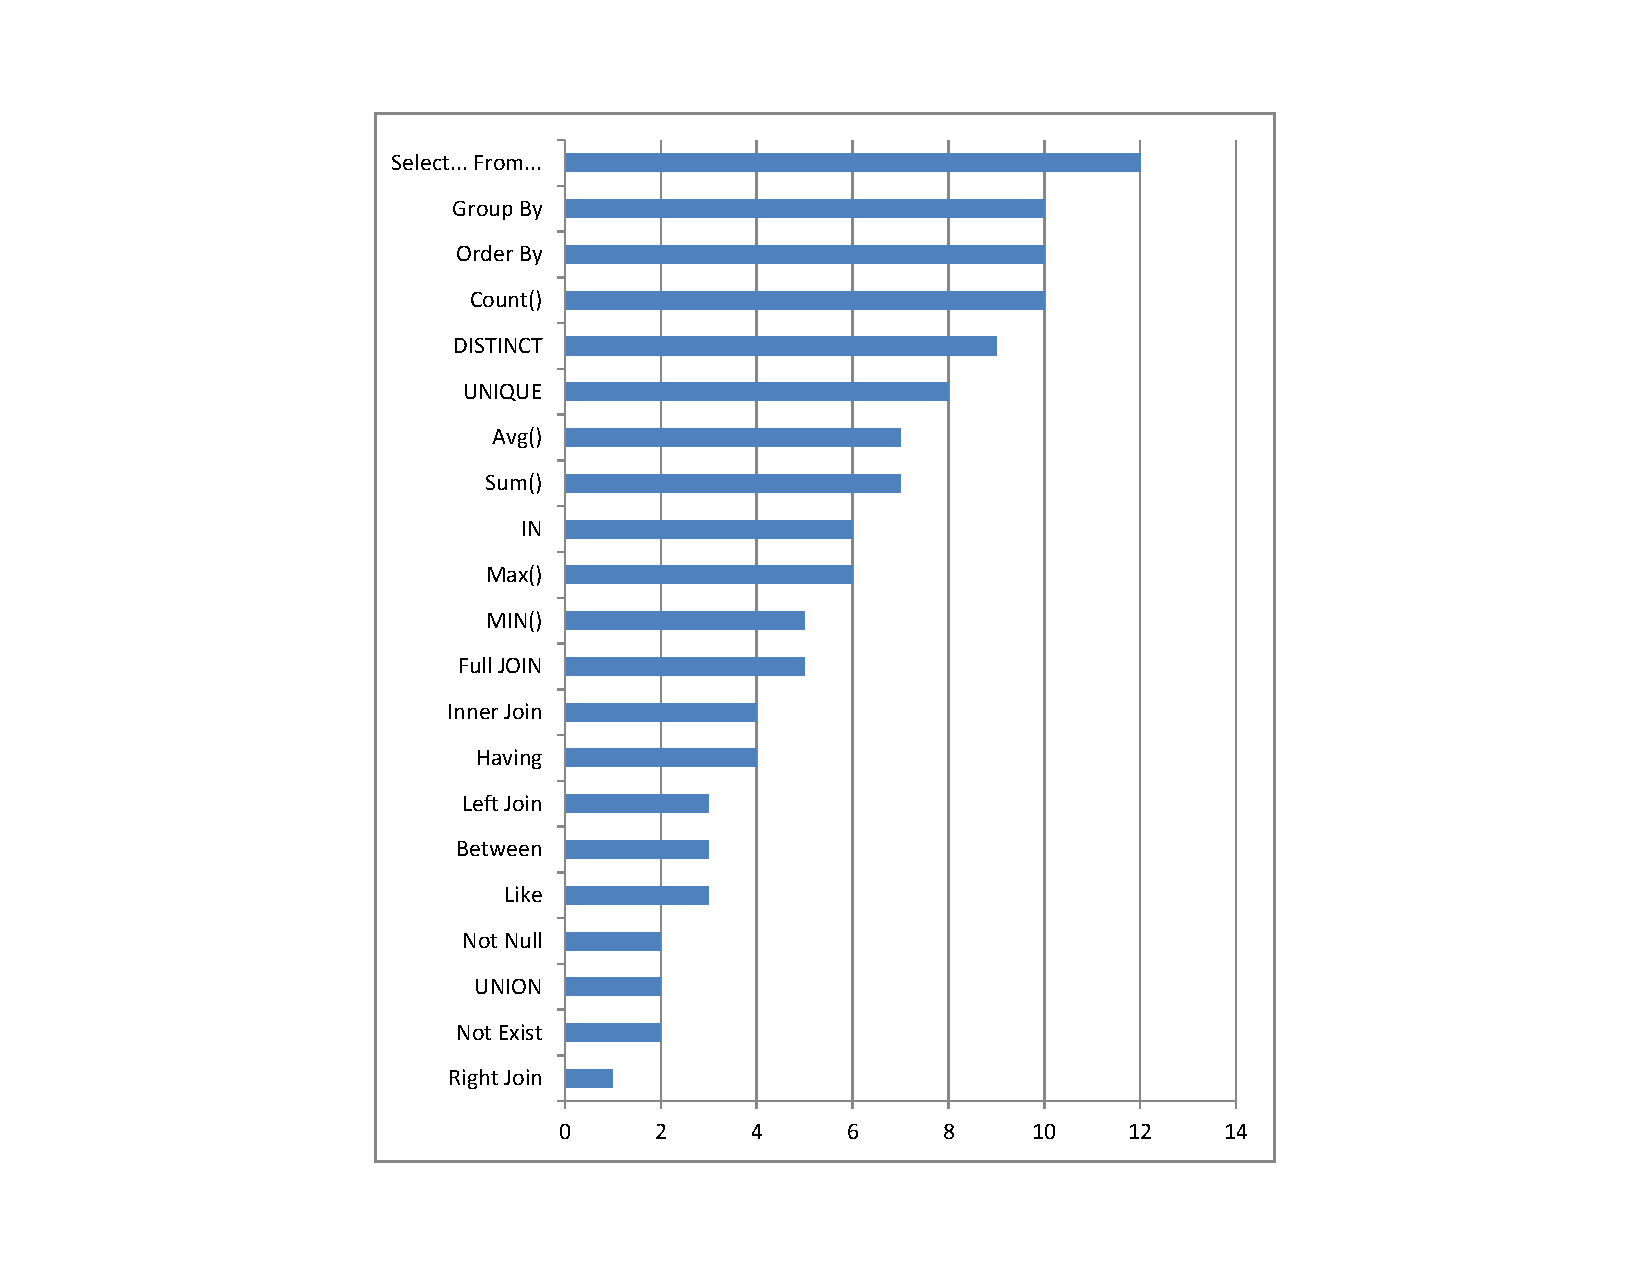
\includegraphics[scale=0.55]{survey}
  \vspace*{-3.0ex}\caption {{\label{fig:survey}
  Survey results of the most widely-used SQL features
  in writing a database query. Each participant
  selected the top 10 most common SQL features.
 % There were 12 participants
 % in the survey, and each participant was asked to
 % select the top 10 widely-used SQL features.
  SQL features with no vote are omitted 
  for brevity.
}}
\vspace{-1mm}
\end{figure}

\newcommand{\q}{\langle query\rangle}
\newcommand{\db}{\langle db\rangle}
\newcommand{\pat}{\langle pat\rangle}
\newcommand{\bug}{\langle bug\rangle}
\newcommand{\dist}{\langle distance\rangle}
\newcommand{\sem}[1]{\llbracket #1\rrbracket}
\newcommand{\lit}[1]{\texttt{#1}}

\newcommand{\column}{\langle column\rangle}
\newcommand{\dbtable}{\langle table\rangle}
\newcommand{\cond}{\langle cond\rangle}
\newcommand{\op}{\langle op\rangle}
\newcommand{\e}{\langle expr\rangle}
\newcommand{\ce}{\langle cexpr\rangle}

\begin{figure}[t]
%\scriptsize{%
\footnotesize%
\begin{align*}
\q ::= {} 
	& \texttt{ SELECT } \e^+ \texttt{ FROM } \dbtable^+ \\
        & \texttt{ WHERE } \cond^+ \\ 
	&  \texttt{ GROUP BY } \column^+ \texttt{ HAVING } \cond^+\\
	&  \texttt{ ORDER BY } \column^+ \\
\dbtable::= {} &\ atom \\
\column ::= {} &\ \dbtable.atom\\
\cond ::= {} &\ \ \cond \;\texttt{\&\&}\; \cond \\ 
    & |\ \cond \;\texttt{||}\; \cond \\
    & |\ \texttt{(}\;\cond\;\texttt{)} \\
    & |\ \ce \;\op\; \ce \\
\op ::= {} &\ \ \texttt{=} \;\;|\;\; \texttt{>}  \;\;|\;\; \texttt{<}\\
\ce ::= {} &\ \ const \;\;|\;\; \column  \;\; \\
\e ::= {} & \ce \;\;|\ \texttt{COUNT}(\column) \;\;|\ \texttt{COUNT}(\texttt{DISTINCT}\;\column)\\
    & |\ \texttt{SUM}(\column) \;\;|\ \texttt{MAX}(\column) \;\;|\ \texttt{MIN}(\column) 
\end{align*}
\normalsize%
\caption{Syntax of the supported SQL subset in \ourtool:
\textit{const} is a constant value and
\textit{atom} is a string value, representing
a table name or a column name.
%This subset covers the top XXX \todo{refer to figure 2}
%in Figure~\ref{fig:survey}
}
\label{fig:syntax}
\vspace{-.5mm}
\end{figure}


\section{A SQL Subset Supported in \ourtool}
\label{sec:langsubset}

\vspace{-1mm}

%The problem of finding a SQL query satisfying
%an example input and output pair is PSPACE-hard~\cite{DasSarma:2010}. 
%To make it tractable,
%instead of supporting all features in the standard
%SQL language, 
\ourtool focuses on a widely-used SQL subset
using which a large class of query tasks can be performed.
Unfortunately, when designing the SQL
subset, we found that no empirical
study has ever been conducted to this end,
and little evidence has ever been provided
on which SQL features are widely-used in practice.
Without such knowledge, deciding which
SQL subset to support remains difficult.


To address this challenge and reduce our personal bias
in designing the language subset, we first conducted an online survey
to ask experienced IT professionals about the most widely-used
SQL features in writing database queries (Section~\ref{sec:survey}).
Then, based on the survey results, we designed
a SQL subset (Section~\ref{sec:syntax}).  
Later, we sent the designed SQL subset to the survey participants
and conducted a series of follow-up email interviews
to confirm whether our design would be sufficient in practice.




%Identify a domain of data on which a large class of users struggle to perform repetitive operations that they can clearly describe with examples





\vspace{-1mm}
\subsection{Online Survey: Eliciting Design Requirements}
\label{sec:survey}

\vspace{-1mm}

Our online survey consists of 6 questions that can be
divided into two parts. The first part includes
demographic information including experience in using SQL.
In the second part, participants were asked to select
the top 10 most widely-used SQL features in their minds.
Instead of directly asking participants about the SQL
features, which might be vague and difficult to respond,
we present them a list of \textit{all} standard
SQL features in writing a query.

%Before distributing our survey, we conducted pilot
%interviews with three graduate students with XXX experience
%at University of Washington. We ran the survey with them and
%made notes of their comments. According to their feedback,
%we refined the survey questions and adjusted the wording to
%make sure that the questions are relevant and clear.


We posted our survey on
professional online forums (e.g., StackOverflow)
and sent to graduate students at University of Washington.
As of April 2013, we received \respnum responses.
On average, the respondents had 9.5 years of experience
in software development (max: 15, min: 5),
and 5.5 years of experience in
using databases (max: 10, min: 2). In addition, two
participants identified themselves as database professionals.
Figure~\ref{fig:survey} summaries the survey results.
% about
%the most-widely used SQL features rated by 12 participants.

\vspace{-1mm}
\subsection{Language Syntax}
\label{sec:syntax}
\vspace{-1mm}

Based on the survey results, we designed a subset
of the standard SQL language, whose
syntax is shown in Figure~\ref{fig:syntax}.
%Its semantics are the same as the standard SQL language,
%and are omitted here for brevity.
%shown in
%that can contains
%many widely-used features required by real users. 
% shows the language syntax.


The supported SQL subset covers all top 10 most widely-used SQL
features voted by the survey participants
in Figure~\ref{fig:survey}, except for the \CodeIn{IN} keyword.
In addition, the SQL subset supports the \CodeIn{HAVING}
keyword since \CodeIn{HAVING} is often used together with the \CodeIn{GROUP BY} clause.
Our SQL subset, though by no means complete in writing all
possible queries, has significantly
enriched the SQL subsets supported by the existing query inference
work~\cite{DasSarma:2010, Tran:2009}. Besides being able to write
standard select-from-where queries as in~\cite{DasSarma:2010, Tran:2009},
our SQL subset also supports table joins, aggregates
(e.g., \CodeIn{COUNT}, \CodeIn{MAX}, \CodeIn{MIN}, and \CodeIn{AVG}),
the \CodeIn{GROUP BY} clause, the \CodeIn{ORDER BY} clause,
and the \CodeIn{HAVING} clause. For readers who are not
familiar with the basic SQL idioms, Figure~\ref{fig:queryex}
shows an example query using our SQL subset.


When designing the SQL subset, we focused on standard
SQL features and excluded user-defined functions and
vendor-specific features, such as the \CodeIn{TOP}
keyword supported in Microsoft SQLServer. 
We discarded some standard SQL features, primarily for
three reasons. First, some features are designed
as syntactic sugar to make a SQL query easier to write;
and thus can be safely removed without affecting a language's
functionality. For example, the \CodeIn{BETWEEN}
keyword checks whether a given value is within a specific
range or not, and can be simply replaced by two query conditions.
Similarly, the \CodeIn{NOT NULL} keyword is also omitted.
%and \CodeIn{LIKE} keywords are also discarded.
Second, some features, such as 
\CodeIn{FULL JOIN}, \CodeIn{LEFT JOIN}, and \CodeIn{RIGHT JOIN},
provide special ways to join tables, and are less likely to be
used by non-expert end-users.
Third, other features, such as \CodeIn{IN} and \CodeIn{NOT EXIST},
are used to write sub-queries or nested queries, which are the major sources
of the PSPACE-hardness in query inference~\cite{DasSarma:2010}.
Related, the \CodeIn{LIKE} keyword is designed for string
wildcard matching; determining its matching
patterns requires systematic search and can be
expensive in practice. Thus, 
for the sake of inference efficiency, we excluded these keywords.

%would quickly become intractable during 
%pattern matching
%and can introduce unmanageable overhead during inference. 
%in order to make the synthesis problem more tractable.

%is also discarded, since it is used for
%string wildcard matching, and can also lead to \todo{xx}

%designed for 
%for the sake of The \CodeIn{LIKE}
%keyword is designed for string wildcard matching rather than
%table query. We also exclude it in the SQL subset


\begin{figure}[t]
  \centering
  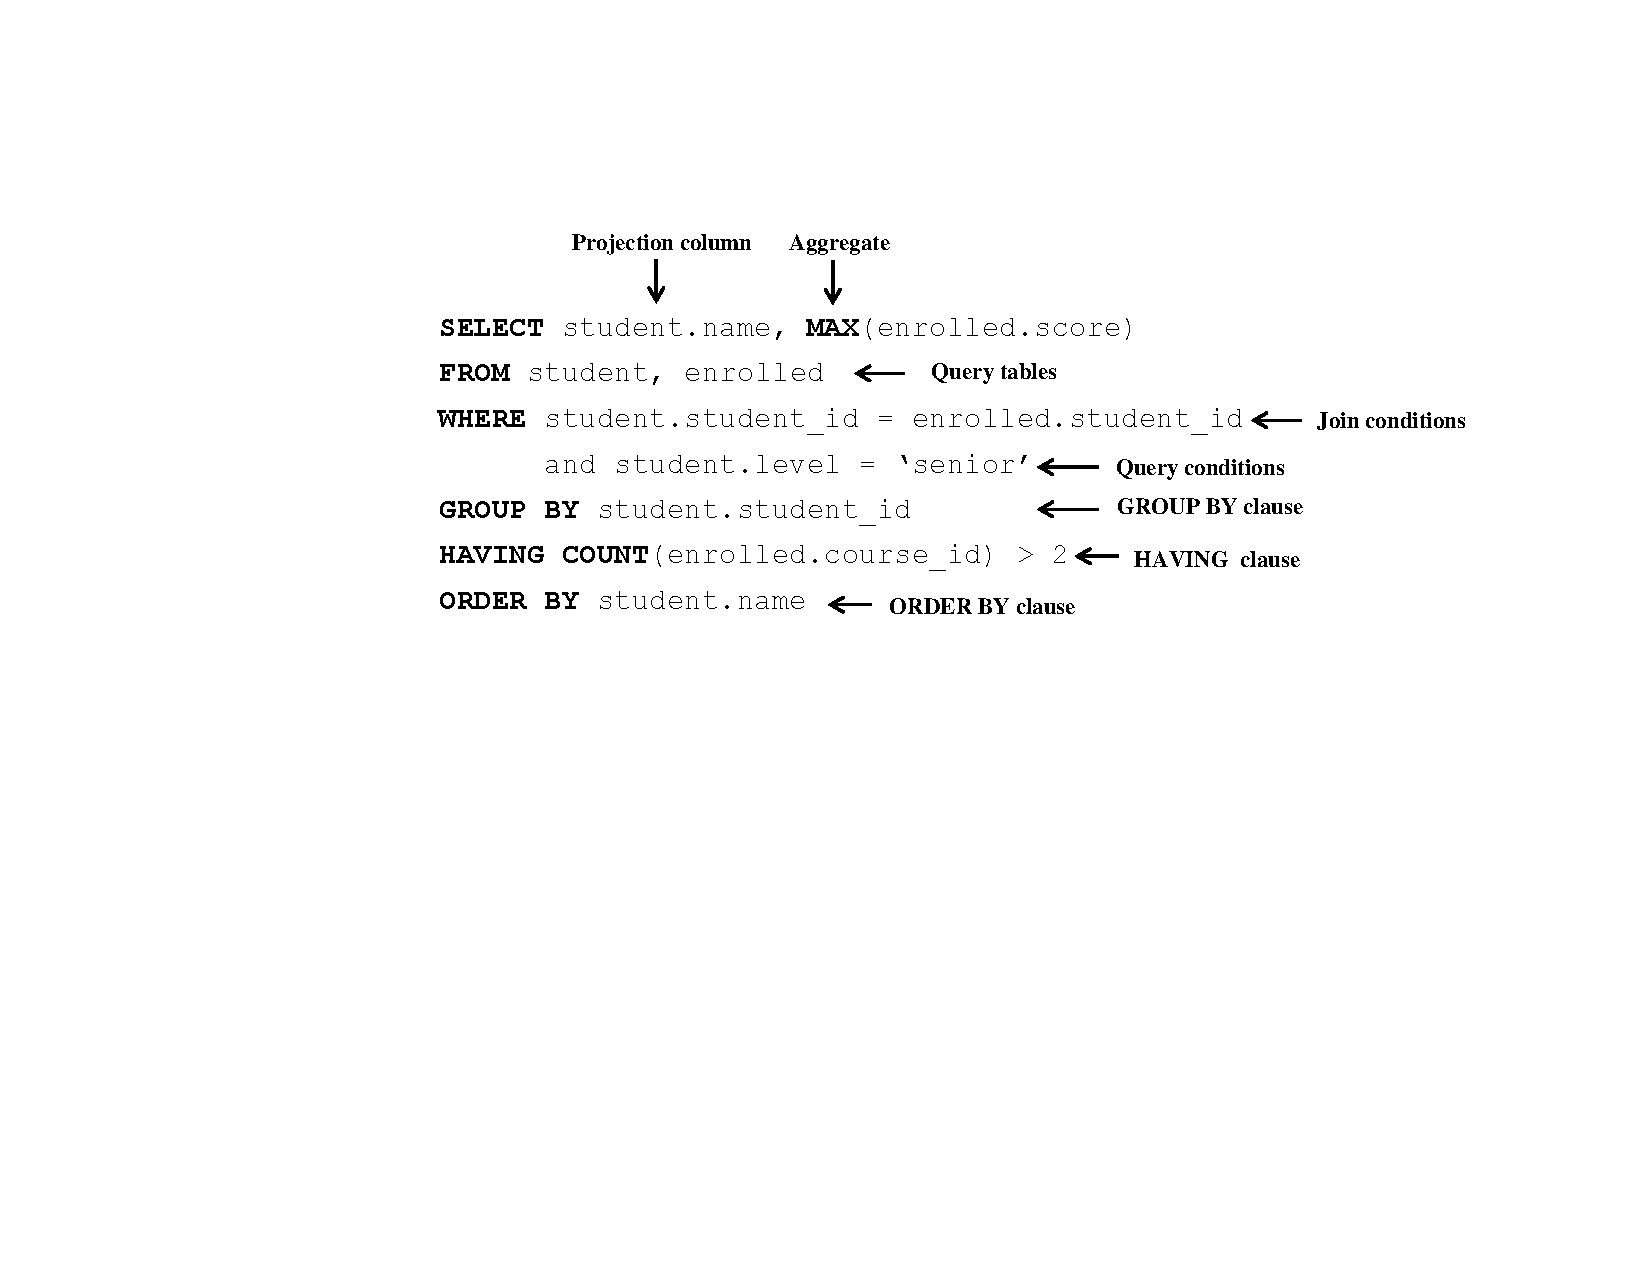
\includegraphics[scale=0.52]{queryex}
  \vspace*{-5.3ex}\caption {{\label{fig:queryex}
  An example query using the SQL subset defined in Figure~\ref{fig:syntax}.
}}
\end{figure}

\vspace{-1mm}

\subsection{Follow-up Interviews: Feedback about the SQL Subset}
\label{sec:interview}

\vspace{-1mm}

After proposing the SQL subset in Figure~\ref{fig:syntax},
we performed follow-up email interviews to gain
participants' feedback. Participants were first asked to rate
the sufficiency of the SQL subset in Figure~\ref{fig:syntax}
in writing real-world database queries,
on a 6-point scale (5-completely
sufficient; 0-not sufficient at all;
and in-between values indicating intermediate sufficiency),
and then to provide their comments.

The average rating of the proposed SQL subset is 4.5. Most of
the participants rated it 5, or 4. Only one participant rated
it 3, because this participant misinterpreted the language
syntax and thought it does not support table joins.
%One participant commented that the SQL subset did not support
%column re-naming. However, re-naming database columns is not
%critical in sythesizing a correct SQL query \todo{xxx}

Overall, based on the feedback by experienced IT professionals,
we believe our SQL subset is usable
for end-users in writing common database queries.
%contains adequate SQL features
%in writing database queries that most end-users need.

